%!TEX root = ../main.tex
\section{Bisimulations and Games}\label{sec:games}
\noindent \textbf{Bisimulations for guarded fragments.}
%
We next present notion of bisimulation relations tailored towards $\GF$ and $\FGF$, based on presentations from~\cite[Sec. 2.2.3]{Otto04} and~\cite[Sec. 2]{BednarczykJ22}.

For structures $\str{A}$ and $\str{B}$ we denote with $\PartIso{\str{A}}{\str{B}}$ the set of all partial isomorphisms between $\str{A}$ and $\str{B}$.
For non-empty $\bisimY, \bisimZ \subseteq \PartIso{\str{A}}{\str{B}}$ we say that $\bisimZ$ satisfies back-and-forth conditions for $\bisimY$ if for every partial isomorphism $\partisof \in \bisimY$ we have:
%
\begin{description}\itemsep0em
  \item[\desclabel{(Forth)}{bisim:forth}] For every live $\elemtuplea$ in $\str{A}$, there is $\partisog \in \bisimZ$ with the domain $\set(\elemtuplea)$ such that $\partisof$ and $\partisog$ agree on their common domain.
  \item[\desclabel{(Back)}{bisim:back}] For every live $\elemtupleb$ in $\str{B}$, there is $\partisog \in \bisimZ$ with the image $\set(\elemtuplea)$ such that $\partisof$ and $\partisog$ agree on their common image.
\end{description}
A non-empty set $\bisimZ \subseteq \PartIso{\str{A}}{\str{B}}$ is a $\GF$-\emph{bisimulation} between $\str{A}$ and $\str{B}$ if it itself satisfies \ref{bisim:forth} and~\ref{bisim:back} conditions given above.
An $\ell$-$\GF$-bisimulation between $\str{A}$ and $\str{B}$ is a sequence of sets $\bisimZ_0, \bisimZ_1, \ldots, \bisimZ_\ell \subseteq \PartIso{\str{A}}{\str{B}}$ such that for all $i < \ell$ we have that $\bisimZ_i$ satisfies~\ref{bisim:forth} and~\ref{bisim:back} conditions for $\bisimZ_{i{+}1}$.
We say that pointed structures $(\str{A}, \elemtuplea)$ and~$(\str{B}, \elemtupleb)$ are $\GF$-\emph{bisimilar}, denoted $(\str{A}, \elemtuplea) \bisimto_{\GF} (\str{B}, \elemtupleb)$, if there exists a $\GF$-bisimulation between $\str{A}$ and $\str{B}$ containing the partial isomorphism that maps $\elemtuplea$ to $\elemtupleb$.
We analogously speak about $\ell$-$\GF$-\emph{bisimilarity} and employ the notation $(\str{A}, \elemtuplea) \bisimto_{\GF}^{\ell} (\str{B}, \elemtupleb)$.
We use the notation $\elemtuplea \bisimto_{\GF} \elemtupleb$ or $\elemtuplea \bisimto_{\GF}^{\ell} \elemtupleb$ if the structures $\str{A}$ and $\str{B}$ are clear from the context.

The following classical lemma links bisimulations and logical~equivalence.
\begin{lemma}[Thm. 1.12 of~\cite{Gradel014}]\label{lemma:GF-bisimulations-work-well}
For every pair of pointed structures $(\str{A}, \elemtuplea)$ and~$(\str{B}, \elemtupleb)$ we have that:
\begin{enumerate}[(a)]
\item $(\str{A}, \elemtuplea) \bisimto_{\GF} (\str{B}, \elemtupleb)$ implies $(\str{A}, \elemtuplea) \equiv_{\GF} (\str{B}, \elemtupleb)$;
\item $(\str{A}, \elemtuplea) \bisimto_{\GF}^{\ell} (\str{B}, \elemtupleb)$ implies $(\str{A}, \elemtuplea) \equiv_{\GF_\ell} (\str{B}, \elemtupleb)$ for all $\ell \in \N$;
\end{enumerate}
Moreover, the converse holds for $\omega$-saturated $\str{A}$ and $\str{B}$.
\end{lemma}

The following example presents $\GF$-bisimilar structures that can be distinguished by a first-order formula.
\begin{example}
  Consider an $\FO[\{\relE\}]$-formula $\varphi \deff \exists{x_{1}, x_{2}, x_{3}}(\relE(x_{1}, x_{2}) \land \relE(x_{2}, x_{3}) \land \relE(x_{3}, x_{1}))$, and structures $\str{A}$, and $\str{B}$ depicted below.
  \begin{figure}[H]
  \centering
  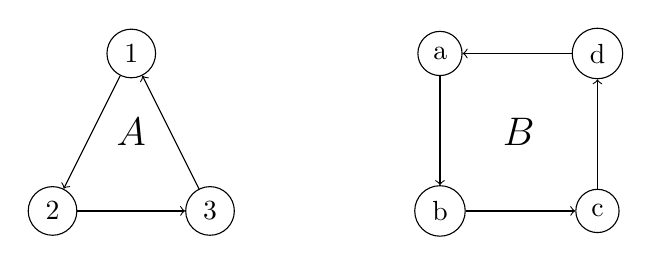
\begin{tikzpicture}[every node/.style={draw,circle}, baseline=(current bounding box.north)]
    \begin{scope}[xshift=-70]
    \node[draw=none, font=\Large] {$\str{A}$};
    \path[->]
      (0,1) node(n1) {1}
      (-1,-1) node(n2) {2}
      (1,-1) node(n3) {3}
      (n1) edge (n2)
      (n2) edge (n3)
      (n3) edge (n1);
    \end{scope}

    \node[draw=none, font=\Large] {$\bisimto_{\GF}$};

    \begin{scope}[xshift=70]
    \node[draw=none, font=\Large] {$\str{B}$};
    \path[->]
      (-1,1) node(n1) {a}
      (-1,-1) node(n2) {b}
      (1,-1) node(n3) {c}
      (1,1) node(n4) {d}
      (n1) edge (n2)
      (n2) edge (n3)
      (n3) edge (n4)
      (n4) edge (n1);
    \end{scope}
  \end{tikzpicture}
  \end{figure}
  By design we clearly have $\str{A}\models \varphi$ and $\str{B} \not\models \varphi$. On the other hand, $\str{A}$ and $\str{B}$ are $\GF$-bisimilar, witnessed by the bisimulation $\bisimZ$ consisting of the partial isomorphisms:
  \begin{itemize}
    \item $s_{1} \mapsto t_{1}$ for every $s_{1} \in \{1,2,3\}$ and $t_{1} \in \{a,b,c,d\}$, and
    \item $s_{1}s_{2} \mapsto t_{1}t_{2}$ for every $s_{1}s_{2} \in \{12,23,31\}$ and $t_{1}t_{2} \in \{ab,bc,cd,da\}$
  \end{itemize}
  where $s_{1}s_{2} \mapsto t_{1}t_{2}$ denotes the partial isomorphism mapping the element $s_{1}$ to $t_{1}$ and the element $s_{2}$ to $t_{2}$.
\end{example}

\noindent
Now a similar characterisation can be provided for $\FGF$.
Due to the ``forwardness'' of the underlying logic, it is convenient to think about maps as tuples.
A \emph{system of forward partial maps} between structures $\str{A}$ and $\str{B}$ is any non-empty subset of $\bigcup_{i=1}^{\infty} (A^i \times B^i)$ satisfying:
\begin{description}\itemsep0em
  \item[\desclabel{(AtomicEq)}{bisim:atomiceq}] For all $(\elemtuplea, \elemtupleb) \in \bisimZ$ we have that $\elemtuplea$, $\elemtupleb$ are live and $\atp{\FGF}{\str{A}}{\elemtuplea} = \atp{\FGF}{\str{B}}{\elemtupleb}$~holds.
\end{description}
For our fixed signature $\Sigma$, the infinite union $\bigcup_{i=1}^{\infty} (A^i \times B^i)$ in this definition may be replaced by the finite union $\bigcup_{i=1}^{\arity(\Sigma)} (A^i \times B^i)$, since live tuples cannot have more than $\arity(\Sigma)$ components.
If $\bisimZ, \bisimZ'$ are systems of forward partial maps between $\str{A}$ and $\str{B}$, we say that $\bisimZ'$ satisfies back-and-forth conditions for $\bisimZ$ if for every $(\elemtuplea, \elemtupleb) \in \bisimZ$ the following conditions hold:
\begin{description}\itemsep0em
  \item[\desclabel{(fForth)}{bisim:fforth}] For every (possibly empty) infix $\elemtuplecfromto{i}{j}$ of $\elemtuplec$ and a live tuple $\elemtuplee$ in $\str{A}$ such that $\elemtuplecfromto{i}{j} = \elemtupleefromto{1}{j{-}i{+}1}$ there is a live tuple $\elemtuplef$ with $\elemtupledfromto{i}{j} = \elemtupleffromto{1}{j{-}i{+}1}$ such that $(\elemtuplee, \elemtuplef) \in \bisimZ'$ holds.
  %
  \item[\desclabel{(fBack)}{bisim:fback}] For every (possibly empty) infix $\elemtupledfromto{i}{j}$ of $\elemtupled$ and a live tuple $\elemtuplef$ in $\str{B}$ such that $\elemtupledfromto{i}{j} = \elemtupleffromto{1}{j{-}i{+}1}$ there is a live tuple $\elemtuplee$ with $\elemtuplecfromto{i}{j} = \elemtupleefromto{1}{j{-}i{+}1}$ such that $(\elemtuplee, \elemtuplef) \in \bisimZ'$~holds.
\end{description}
A system of forward partial maps $\bisimZ$ between $\str{A}$ and $\str{B}$ is an $\FGF$-\emph{bisimulation} between $\str{A}$ and $\str{B}$ if it itself satisfies the above conditions.
An $\ell$-$\FGF$-bisimulation between $\str{A}$ and $\str{B}$ is a sequence $\bisimZ_0, \bisimZ_1, \ldots, \bisimZ_\ell$ of systems of forward partial maps between $\str{A}$ and $\str{B}$ such that for all $i < \ell$ we have that $\bisimZ_i$ satisfies~\ref{bisim:fforth} and~\ref{bisim:fback} conditions for $\bisimZ_{i{+}1}$.
We~speak about $\FGF$-\emph{bisimilar} and $\ell$-$\FGF$-\emph{bisimilar} (pointed) structures in total analogy to the guarded-fragment case.
We stress that the back-and-forth conditions allow for choosing an empty infix, so $\ell$-$\FGF$-bisimulations are not limited to the local neighbourhood of some tuple.
Instead, even for $\ell = 1$, every guarded tuple must be mapped to a tuple in the other structure.

A ``forward'' counterpart of \cref{lemma:GF-bisimulations-work-well} is presented below.
\begin{lemma}\label{lem:FGF-bisimulations-work-well}
For every pair of pointed structures $(\str{A}, \elemtuplea)$ and~$(\str{B}, \elemtupleb)$ we have that:
\begin{enumerate}[(a)]
\item $(\str{A}, \elemtuplea) \bisimto_{\FGF} (\str{B}, \elemtupleb)$ implies $(\str{A}, \elemtuplea) \equiv_{\FGF} (\str{B}, \elemtupleb)$;
\item $(\str{A}, \elemtuplea) \bisimto_{\FGF}^{\ell} (\str{B}, \elemtupleb)$ implies $(\str{A}, \elemtuplea) \equiv_{\FGF_\ell} (\str{B}, \elemtupleb)$ for all $\ell \in \N$;
\end{enumerate}
Moreover, the converse holds for $\omega$-saturated $\str{A}$ and $\str{B}$.
\end{lemma}
\begin{proofsketch}
  A proof for condition \textbf{(a)} is provided in~\cite[Lemma 3]{BednarczykJ22}.
  The proof for condition \textbf{(b)} uses the same ideas as the proof for \textbf{(a)}.
  \begin{itemize}
    \item
          For the ``if'' direction, we perform induction over $\ell$ and use~\ref{bisim:fforth} to obtain a witness in $\str{B}$ for every existential quantifier that has a witness in $\str{A}$ (by properties of $\models$, it suffixes to consider existential quantifiers as $\forall\vartuplex\ \cdots \iff \lnot \exists \vartuplex\ \cdots$).
    \item
          For the opposite direction, we show that the set of pairs of tuples from $\str{A}$ and $\str{B}$ with the same $\FGF_{\ell}$-type is an $\ell$-$\FGF$-bisimulation.
          Let $\elemtuplec \sqin A$ and $\elemtupled \sqin B$ be live tuples with equal $\FGF_{\ell}$-types.
          Consider any tuple $\elemtuplee$ extending an infix $\elemtuplecfromto{i}{j}$ to a new live tuple $\elemtuplecfromto{i}{j}\elemtuplee$.
          Let $\Gamma$ be the $\FGF_{k-1}$-type of $\elemtuplee$ with regards to $\elemtuplecfromto{i}{j}$.
          Because of $\omega$-saturation, this type is realized in $\str{B}$ if every of its finite subsets is realized.
          For every finite subset of $\Gamma$, we can construct an $\FGF_{k}$-formula that asserts the existence of a witness realizing this finite $\FGF_{k-1}$-type.
          Hence by $k$-$\FGF$-equivalence, there exists a tuple $\elemtuplef$ that extends $\elemtupledfromto{i}{j}$ and same $\FGF_{k-1}$-type.
          Therefore, the set of pairs of tuples with equal $\FGF_{\ell}$-types is an $\ell$-$\FGF$-bisimulation, satisfying the theorem.
  \end{itemize}
\end{proofsketch}
../../Lipics version/proofs/FGF-bisimulations-work-well.tex

\noindent
The following example presents two structures that are $\FGF$-bisimilar but not $\GF$-bisimilar.
\begin{example}
  Consider the two structures $\str{A} := \tikz[baseline=-0.5ex]{\path[->] (0,0) node[draw,circle] (n1) {} (n1) edge[loop above,in=70,out=110,looseness=10] (n1);}$ and $\str{B} := \tikz[baseline=-0.5ex]{\path[->] (0,0) node (n1) [draw,circle] {} (3em,0) node (n2) [draw,circle] {} (n1) edge[bend left] (n2) (n2) edge[bend left] (n1);}$ with a binary predicate $\relE$ interpreted as the edge relation. These two structures are $\FGF[\{\relE\}]$-bisimilar, while a $\GF$-sentence $\exists{\varx_1}\relE(\varx_1,\varx_1)$ can distinguish them.

\end{example}

\noindent \textbf{Bisimulation games.}
Both $\GF$-bisimulation and $\FGF$-bisimulation naturally correspond to games~\cite[Sec. 1.2.1]{Gradel014}.
We focus on the the game corresponding to $\FGF$-bisimulation here.
The $\FGF$-\emph{bisimulation game} is played on two pointed structures $(\str{A}, \elemtuplea)$ and $(\str{B}, \elemtupleb)$ by two players, Spoiler and Duplicator.
The game starts by selecting the tuples $\elemtuplea$ and $\elemtupleb$ from the corresponding structures.
Throughout the game, Duplicator must maintain the condition that the two currently selected tuples have equal atomic-$\FGF$-types.
If $\elemtuplea$ and $\elemtupleb$ already do not have the same atomic $\FGF$-type, then Duplicator loses instantly.
Otherwise, the game proceeds in rounds.
In each round, Spoiler first chooses a structure.
As the game is symmetric, let us assume that spoiler chooses the structure $\str{A}$.
Spoiler then selects an infix $\elemtupleafromto{i}{j}$ of the currently selected tuple and a new live tuple $\elemtuplec$ which has $\elemtupleafromto{i}{j}$ as a prefix.
For convenience, we use the terms \emph{shared elements} for the prefix $\elemtuplecfromto{1}{j-i+1}$ and \emph{unshared elements} for the remaining elements, namely $\elemtuplecfromto{j-i+1+1}{|\elemtuplec|}$.
Duplicator, in order to continue the game, must then find a live tuple $\elemtupled$ in $\str{B}$ having $\elemtuplebfromto{i}{j}$ as prefix such that $\elemtuplec$ and $\elemtupled$ have equal $\FGF$-types.
Note that Spoiler may choose an index $j$ that is not maximal, so that the situation of $a_{j+1} = c_{j-i+1+1}$ is still possible.
We still regard $c_{j-i+1+1}$ as an unshared element, since Duplicator is allowed to pick a tuple $\elemtupled$ where $b_{j+1} \neq d_{j-i+1+1}$.
The game then continues with the next round, with $\elemtuplec$ and $\elemtupled$ as the new starting tuples.
Spoiler wins the game if Duplicator is unable to respond, i.e.\ to find suitable tuples.
Duplicator wins otherwise.
It is easy to see that the possible moves of Spoiler are analogous to the back-and-forth conditions for $\FGF$-bisimulation, as is also the case for the $\GF$-game~\cite[Sec.\ 3.2]{Gradel014}.
To win, Duplicator must be able to respond to any move that Spoiler makes.
A winning strategy for Duplicator thus corresponds to an $\FGF$-bisimulation between the two structures, and vice-versa.
If we restrict the game to only $\ell$-rounds, where the winning condition for Duplicator is that Spoiler cannot win in the first $\ell$-rounds, then the game is equivalent (in the aforementioned sense) to the existence of an $\ell$-FGF-bisimulation between $\str{A}, \elemtuplea$ and $\str{B}, \elemtupleb$.
We collect these observations in the following corollary:

\begin{corollary}
  In the $\FGF$-game played on structures $\str{A}, \elemtuplea$ and $\str{B}, \elemtupleb$:
  \begin{itemize}
    \item Duplicator has as winning strategy if and only if $\str{A}, \elemtuplea \bisimto_{\FGF} \str{B}, \elemtupleb$,
    \item Duplicator has a winning strategy for $\ell$ rounds if and only if $\str{A}, \elemtuplea \bisimto_{\FGF}^{\ell} \str{B}, \elemtupleb$.
  \end{itemize}
\end{corollary}

\noindent \textbf{Biseqs and Bipoints.}
We next define two concepts (biseqs and bipoints) which represent a sequence of moves that Spoiler takes and the elements that Spoiler selects, respectively, in one of the possible plays of the $\FGF$-bisimulation game.
Later, in \cref{sec:unraveling}, we employ these concepts to characterize a structure in terms of its behavior under the game.

Let $\str{A}, \elemtuplea^{(0)}$ be a pointed structure where $\elemtuplea^{(0)}$ is just tuple of elements from $A$, labelled with a zero index as it is the start of a sequence of tuples selected by Spoiler.
An $\ell$-\emph{biseq} is a word in $A^*{(\N\N{}A^{*})}^{\ell}$, written as a sequence of the form $\elemtuplea^{(0)}(i^{(1)}, j^{(1)})\elemtuplea^{(1)}\cdots(i^{(\ell)}, j^{(\ell)})\elemtuplea^{(\ell)}$, where each $a^{(k)}$ is a live tuple from $\str{A}$ and $i^{(k)}, j^{(k)}$ are indices with $i \le j$ for which $\elemtupleafromto{i^{(k)}}{j^{(k)}}^{(k-1)} = \elemtupleafromto{1}{j^{(k)}-i^{(k)}+1}^{k}$.
Conceptually, an $\ell$-biseq represents a play of Spoiler in the $\ell$-round $\FGF$-game involving the structure $\str{A}$, where in each round $k$, Spoiler chooses the non-empty infix corresponding to the indices $i^{(k)}\ldots{}j^{(k)}$ and the new tuple $\elemtuplea^{(k)}$.
Biseqs are denoted by greek letters $\rho, \sigma, \theta, \ldots$ and for
a biseq $\sigma$ we refer to the parameter $\ell$ in the above definition as the \emph{level} of $\sigma$.
We say that a biseq $\sigma$ \emph{extends} a biseq $\rho$ if $\sigma$ can be constructed from $\rho$ by adding moves to the end, \ie{} $\rho$ is a prefix of $\sigma$.
The set of all biseqs for a structure $\str{A}$, denoted by $\Seq{A}$, intuitively collects all possible ways in which Spoiler can explore this structure.
For any $\ell$-biseq, if $\str{B}, \elemtupleb^{(0)}$ is a structure that is \FGF-bisimilar to $\str{A}, \elemtuplea^{(0)}$, then we can apply~\ref{bisim:fforth} $\ell$ times to find tuples $\elemtupleb^{1}, \ldots, \elemtupleb^{\ell}$ for a corresponding biseq in $\str{B}$.
The latter sequence represents a possible choice of moves for Duplicator in response to the moves played by Spoiler in the game on the structures $\str{A}, \elemtuplea^{(0)}$ and $\str{B}, \elemtupleb^{(0)}$.
Below are some examples of biseqs:
\begin{figure}[H]
  \centering
    \begin{minipage}[t]{0.2\textwidth}
        \raggedleft%
        \vspace{0pt}
        \includegraphics[scale=0.5]{res/example-struct-1}
    \end{minipage}
    \hspace{4em}
    \begin{minipage}[t]{0.6\textwidth}
      {%
      \newcommand{\tups}{{\color{tolbrightYellowDarker}\elemtuples}}%
      \newcommand{\tupp}{{\color{tolbrightCyanDarker}\elemtuplep}}%
      \newcommand{\tupt}{{\color{tolbrightGreen}\elemtuplet}}%
      \newcommand{\tupq}{{\color{tolbrightPurple}\elemtupleq}}%
      The picture on the left shows a structure with the relations: $(1,2,3) \in \relS^{\str{A}}$, $(2,3,4) \in \relP^{\str{A}}$, $(3,4,5) \in \relT^{\str{A}}$, $(4,5) \in \relQ^{\str{A}}$.

      \vspace{1ex}
      Let $\tups = (1, 2, 3), \tupp = (2, 3, 4), \tupt = (3, 4, 5), \tupq = (4,5)$.

      \vspace{1ex}
      Some examples of biseqs in this structure are:
      \begin{itemize}
          \item $\tups(3,3)\tupt$,
          \item $\tups(2,3)\tupp(2,3)\tupt$.
      \end{itemize}

      Biseqs are not required to use maximal infixes, so the following are also valid biseqs:
      \begin{itemize}
          \item $\tups(2,2)\tupp$,
          \item $\tups(3,3)\tupt(2,2)\tupq$.
      \end{itemize}
      }
    \end{minipage}
    \caption{Examples of biseqs.}%
    \label{fig:biseq-examples}
\end{figure}

Let $\Seq{\str{A}}$ be the set of all biseqs for a structure $\str{A}$.
There is a natural projection $\Pi$ from a biseq $\sigma \in \Seq{A}$ to tuples of $\str{A}$: for $\sigma = \cdots (i,j) \elemtuples$, we define $\Pi(\sigma)$ as $\Pi(\sigma) = \elemtuples$.
Intuitively, this projection gives the tuple of selected elements in structure $\str{A}$ in the bisimulation game after playing the moves of $\sigma$.
We now introduce ``bipoints'', which instead of tuples, project to individual selected elements (``points'') of $\str{A}$.
A \emph{bipoint} of a structure $\str{A}$ is a tuple $(\sigma, k) \in \Seq{A} \times \mathbb{N}$ such that
\begin{itemize}
  \item $\sigma = \elemtuplea$, $k \ge 1$ and $k \le |\elemtuplea|$ for some $\elemtuplea \sqin A$, or
  \item $\sigma = \cdots (i,j) \elemtuplea$, $k \ge (j-i+1) + 1$ and $k \le |\elemtuplea|$ for some $\elemtuplea \sqin A$.
\end{itemize}
For a bipoint $e$ of a structure $A$ that can be decomposed as $e = (\rho, k)$, we use the notation $\seq{e} = \rho$ and $\ctr{e} = k$ to denote the biseq and the counter of this bipoint, respectively.
The counter of the bipoint identifies one component of the tuple of elements that the biseq projects to.
We define the projection $\pi$ from bipoints of a structure $\str{A}$ to elements of $\str{A}$ as: if $e = (\sigma, k)$ is a bipoint, then $\pi(e) = {\Pi(\sigma)}_{k}$ (= $\elema_{k}$ for $\sigma = \cdots\elemtuplea$).
The condition that ``$k \ge (j-i+1) + 1$'' ensures that we do not have more than one bipoint for the shared elements in a move in the bisimulation game.
\cref{ex:bipoints} shows a concrete application for this condition.

\begin{example}\label{ex:bipoints}
   {%
     \newcommand{\tups}{{\color{tolbrightYellowDarker}\elemtuples}}%
     \newcommand{\tupt}{{\color{tolbrightGreen}\elemtuplet}}%
     \newcommand{\es}{{\color{tolbrightYellowDarker}s}}%
     \newcommand{\et}{{\color{tolbrightGreen}t}}%
     Consider the biseqs from \cref{fig:biseq-examples}.
     The bipoints for the 0-biseq $\sigma$ with $\sigma = \tups$ are: $a = (\sigma, 1)$, $b = (\sigma, 2)$ and $c = (\sigma, 3)$.
     These project to the components of the tuple $\tups$: $\pi(a) = \es_{1} = 1$, $\pi(b) = \es_{2} = 2$ and $\pi(c) = \es_{3} = 3$.
     Now consider the 1-biseq $\rho$ with $\rho = \tups(3,3)\tupt$.
     Regarded in terms of the game, this sequence represents the move from $\tups$ to $\tupt$, sharing the element ``3''.
     There are bipoints $d = (\rho, 2)$ and $e = (\rho, 3)$ which project to the domain elements ``4'' and ``5''.
     However, there is no bipoint for the sequence $\rho$ that projects to ``3''.
     While $(\rho, 1)$ projects to ``3'' according to the definition of $\pi$, it is not a bipoint as it violates the ``$k \ge (j-i+1) + 1$'' condition in the above definition.
     Note that $c = (\sigma, 3)$ projects to ``3'', so there already is a bipoint that projects to ``3'', using the sequence $\sigma$.
     In fact, bipoints correspond one-to-one to unshared elements of moves in the bisimulation game.
     From the point of view of the biseq $\sigma$, the element ``3'' is not shared with previously selected elements (there are none, since $\sigma$ represents the start of the game at tuple $\tups$), while relative to the biseq $\rho$, the element ``3'' is among the shared elements.
     Hence, $(\sigma, 3)$ is a bipoint, while $(\rho ,1)$ is not.
   }
\end{example}
